\section{}
\[
H(s)=\frac{s+1}{s^2+2s+1}=\frac{1}{s+1}\,.
\]
\subsection{Bode-Diagramm}
\begin{center}
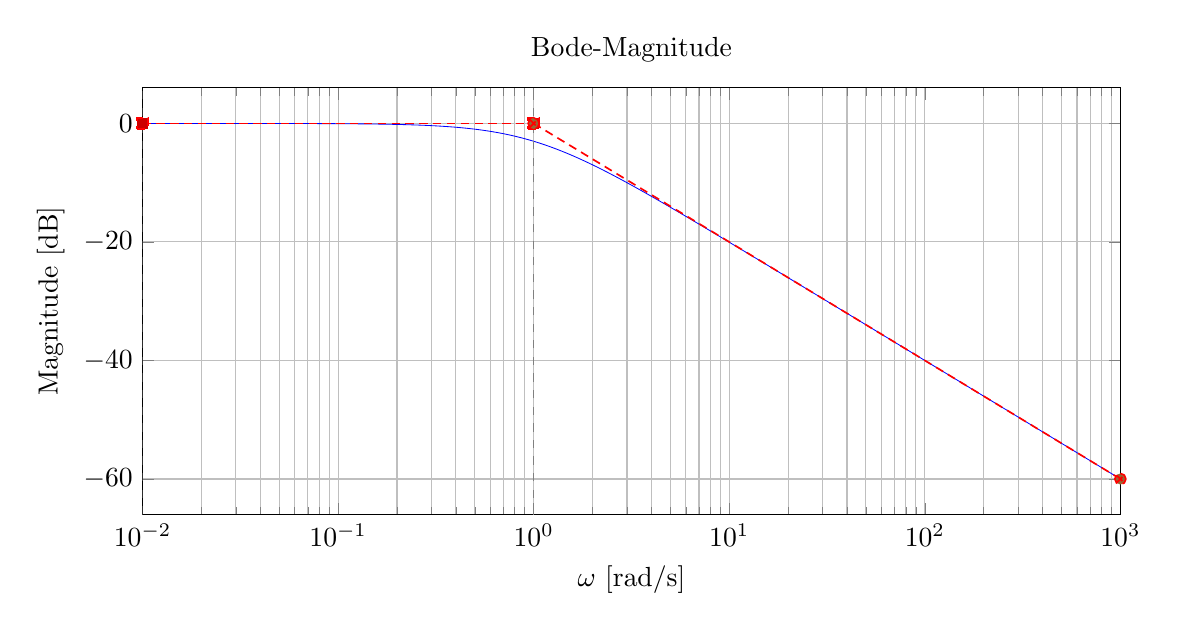
\begin{tikzpicture}
\begin{semilogxaxis}[
  width=14cm,height=7cm,
  xmin=1e-2,xmax=1e3,
  xlabel={$\omega$ [rad/s]},
  ylabel={Magnitude [dB]},
  grid=both,
  ytick distance=20,
  title={Bode-Magnitude}
]
\addplot[
  domain=1e-2:1e3,
  samples=600,
  mark=none,
  line width=0.3pt,
  blue
] {-20*ln(sqrt(1 + x^2))/ln(10)};
\addplot+[domain=1e-2:1,samples=2,dashed,dash pattern=on 3pt off 2pt,line width=0.6pt,red] {0};
\addplot+[domain=1:1e3,samples=2,dashed,dash pattern=on 3pt off 2pt,line width=0.6pt,red] {-20*ln(x)/ln(10)};
\draw[gray,dashed] (rel axis cs:0,0) -- (rel axis cs:0,1);
\draw[gray,dashed] (axis cs:1,\pgfkeysvalueof{/pgfplots/ymin}) -- (axis cs:1,\pgfkeysvalueof{/pgfplots/ymax});
\node[gray,anchor=south east] at (axis cs:1,\pgfkeysvalueof{/pgfplots/ymax}) {\scriptsize Pol $\omega_p=1$};
\end{semilogxaxis}
\end{tikzpicture}
\vspace{6mm}
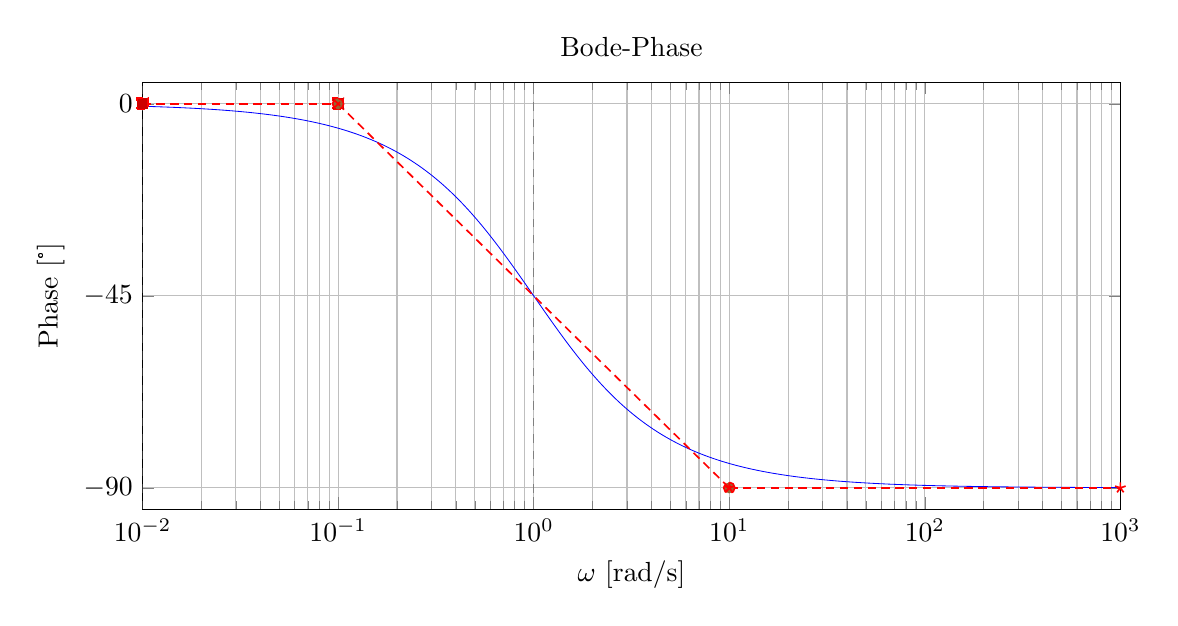
\begin{tikzpicture}
\begin{semilogxaxis}[
  width=14cm,height=7cm,
  xmin=1e-2,xmax=1e3,
  ymin=-95,ymax=5,
  ytick distance=45,
  xlabel={$\omega$ [rad/s]},
  ylabel={Phase [°]},
  grid=both,
  title={Bode-Phase}
]
\addplot[
  domain=1e-2:1e3,
  samples=600,
  mark=none,
  line width=0.3pt,
  blue
] {-atan(x)};
\addplot+[domain=1e-2:1e-1,samples=2,dashed,dash pattern=on 3pt off 2pt,line width=0.6pt,red] {0};
\addplot+[domain=1e-1:1e1,samples=2,dashed,dash pattern=on 3pt off 2pt,line width=0.6pt,red] {-45 - 45*ln(x)/ln(10)};
\addplot+[domain=1e1:1e3,samples=2,dashed,dash pattern=on 3pt off 2pt,line width=0.6pt,red] {-90};
\draw[gray,dashed] (rel axis cs:0,0) -- (rel axis cs:0,1);
\draw[gray,dashed] (axis cs:1,\pgfkeysvalueof{/pgfplots/ymin}) -- (axis cs:1,\pgfkeysvalueof{/pgfplots/ymax});
\node[gray,anchor=south east] at (axis cs:1,\pgfkeysvalueof{/pgfplots/ymax}) {\scriptsize Pol $\omega_p=1$};
\end{semilogxaxis}
\end{tikzpicture}
\end{center}
\newpage
\subsection{Erklärung (ausführlich)}
\begin{description}[leftmargin=1.2em,labelsep=.6em,font=\bfseries]

\item[1. Normalform herstellen.]
Bringe die Übertragungsfunktion exakt in die im Skript definierte Standardform.
\[
H(s)=\frac{1}{s+1}=K_0\cdot\frac{1}{1+sT_p}
\]
mit
\[
K_0=1,\quad r=0,\quad T_p=1.
\]
\[
\underline{F}_1(s)=\frac{1}{1+sT_p}=\frac{1}{1+s}\quad\text{(reelles Polglied 1. Ordnung)}.
\]

\item[2. Eckfrequenz bestimmen und sortieren.]
\[
\omega_p=\frac{1}{T_p}=1\,\mathrm{rad/s}.
\]
Nur diese Eckfrequenz; Sortierung trivial.

\item[3. Startpunkt des Amplitudengangs festlegen (Geradennäherung).]
\[
\omega_{\min}=\omega_p=1,\qquad
F_{\mathrm{dB}}(\omega_{\min})=20\log_{10}\!\big(|K_0 F^*_{ges}(0)|\,\omega_{\min}^{\,r}\big)=0\,\mathrm{dB}.
\]
Ankerpunkt bei \(\omega=1 \,\mathrm{rad/s}\): \(0\,\mathrm{dB}\).

\item[4. Verlauf links vom Startpunkt zeichnen.]
Für \(\omega<1\) horizontale Asymptote bei \(0\,\mathrm{dB}\) (Anfangssteigung \(0\,\mathrm{dB/dec}\), da $r\cdot 20\,\mathrm{dB/dec} =0$).

\item[5. Steigungswechsel an der Eckfrequenz eintragen.]
Ein einfacher Pol bewirkt ab \(\omega_p\) eine Steigungsänderung von \(-20\,\mathrm{dB/dec}\).
\[
|H(j\omega)|_{\mathrm{dB}}\approx -20\log_{10}\omega\quad(\omega\ge 1).
\]
$\rightarrow$ Zeichne eine Gerade mit Steigung $-20 \,\mathrm{dB/dec}$ ab $\omega = 1\,\mathrm{rad/s}$

\item[6. Eckabrundung korrekt berücksichtigen.]
Am Knick \(\omega=\omega_p\) liegt der exakte Betrag um \(-3\,\mathrm{dB}\) unter der Asymptote:
\[
|H(j1)|_{\mathrm{dB}}=-10\log_{10}(1+1)=-10\log_{10}2\approx-3\,\mathrm{dB}.
\]

\item[7. Phasenstartwert festlegen.]
\(K_0F_{ges}(0)>0\), \(r=0\) \(\Rightarrow\) \(\varphi(0)=r\cdot 90^\circ=0^\circ\).

\item[8. Phasenänderung durch das Polglied eintragen.]
Ein reelles Polglied 1. Ordnung erzeugt \(-90^\circ\) über die Übergangsdekade.
\[
\varphi(\omega)\approx
\begin{cases}
0^\circ,& \omega\le 0.1,\\
-45^\circ-45^\circ\log_{10}\omega,& 0.1<\omega<10,\\
-90^\circ,& \omega\ge 10.
\end{cases}
\]

\item[9. Grenzwerte und Konsistenz prüfen.]
DC: \(|H(0)|=1\Rightarrow 0\,\mathrm{dB}\), \(\varphi(0)=0^\circ\).
HF: \(|H(j\omega)|\sim 1/\omega\Rightarrow -20\log_{10}\omega\,\mathrm{dB}\), \(\varphi(\infty)=-90^\circ\).
Pol-/Nullzählung: \(m=0\), \(n=1\Rightarrow (m-n)\cdot90^\circ=-90^\circ\) konsistent.

\end{description}

\subsubsection*{Stückweise Näherungen (für die Skizze)}
\[
|H(j\omega)|_{\mathrm{dB}}\approx
\begin{cases}
0,& \omega\ll 1,\\[2pt]
-10\log_{10}2,& \omega=1,\\[2pt]
-20\log_{10}\omega,& \omega\gg 1,
\end{cases}
\]\[
\varphi(\omega)\approx
\begin{cases}
0^\circ,& \omega\le 0.1,\\[2pt]
-45^\circ-45^\circ\log_{10}\omega,& 0.1<\omega<10,\\[2pt]
-90^\circ,& \omega\ge 10.
\end{cases}
\]

\newpage